

\section{Casos de Uso}
\label{sec:casos_de_uso}

Para o projeto, foram elaborados casos de uso do sistema. Na figura \ref{fig:casos_de_uso}
tem-se o diagrama de casos de uso. Na seção \ref{sec:casos_completos} tem-se os casos de uso
completo-abstrato e completo-concreto, relativo ao diagrama da figura \ref{fig:casos_de_uso}.

\subsection{Diagrama de casos de uso}
\begin{figure}[ht]
 \centering
  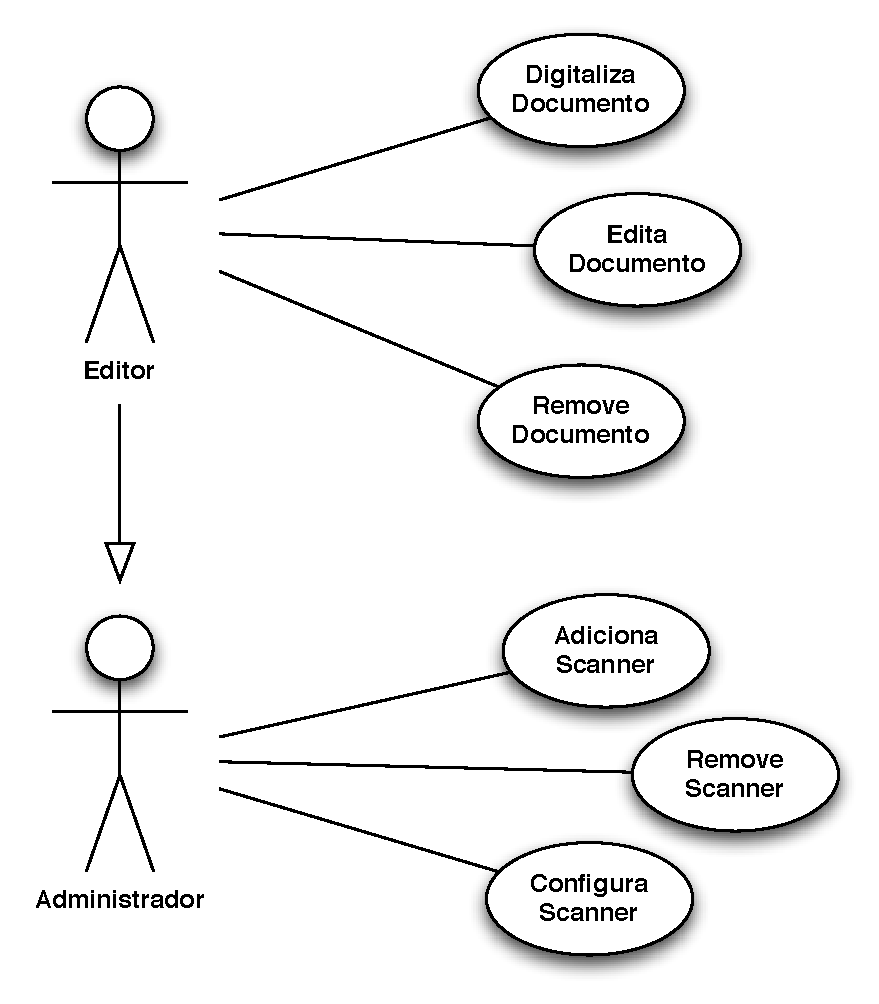
\includegraphics[scale=0.7]{img/use-case-diagram.pdf}
  \caption {Diagramas de casos de uso}
  \label{fig:casos_de_uso}
\end{figure}

\subsection{Casos de uso completos}
\label{sec:casos_completos}

\subsubsection{Caso de uso: Digitaliza documento}
\begin{description}
    \item[{\bf Descrição:}] Nesse caso de uso o ator tem como função colocar um documento no {\it scanner} para digitalizá-lo.
    \item[{\bf Pré-condições:}]
        \begin{enumerate}
            \item Há um documento no {\it scanner};
            \item O {\it scanner} está configurado corretamente;
            \item O {\it scanner} está ligado e funcionando corretamente;
        \end{enumerate}
    \item[{\bf Pós-condições:}] 
        \begin{enumerate}
            \item O documento estará digitalizado;
            \item O documento estará indexado para busca;
        \end{enumerate}

    \item[{\bf Cenário de sucesso:}]
        \begin{enumerate}
            \item O {\it scanner} já foi previamente configurado e está operando corretamente;
            \item O ator colocou um documento no {\it scanner};
            \item O ator ativa o procedimento de digitalização;
            \item O ator muda a página do documento;
            \item O ator realiza os passos 3 e 4 até que todo o documento esteja digitalizado;
            \item O ator decide um nome para o novo documento;
        \end{enumerate}

    \item[{\bf Fluxos alternativos}]
        1 O {\it scanner} não foi configurado ou não está operando; \newline
        (2-8) O {\it scanner} deixa de operar; \newline
        (1-8) O ator desiste da operação; \newline

\end{description}



\subsubsection{Caso de uso: Edita documento}
\begin{description}
    \item[{\bf Descrição:}] Nesse caso de uso o ator tem como função selecionar um documento no sistema para alterar suas características.
    \item[{\bf Pré-condições:}]
        \begin{enumerate}
            \item Há pelo menos um documento digitalizado;
        \end{enumerate}
    \item[{\bf Pós-condições:}] 
        \begin{enumerate}
            \item O documento foi alterado;
        \end{enumerate}
    
    \item[{\bf Cenário de sucesso:}]
        \begin{enumerate}
            \item O ator encontrou o documento;
            \item O ator alterou os dados do documento;
            \item O ator confirmou as alterações;
        \end{enumerate}

    \item[{\bf Fluxos alternativos}]
        1. Não há documentos digitalizados; \newline
        3. O ator não confirmou as alterações;
\end{description}



\subsubsection{Caso de uso: Remove documento}
\begin{description}
    \item[{\bf Descrição:}] Nesse caso de uso o ator tem como função selecionar um documento para ser removido do sistema.
    \item[{\bf Pré-condições:}]
        \begin{enumerate}
            \item Há pelo menos um documento digitalizado;
        \end{enumerate}
    \item[{\bf Pós-condições:}] 
        \begin{enumerate}
            \item O documento foi removido do sistema;
        \end{enumerate}
    
    \item[{\bf Cenário de sucesso:}]
        \begin{enumerate}
            \item O ator encontrou o documento;
            \item O ator acionou a remoção do documento;
            \item O ator confirmou a remoção do documento;
        \end{enumerate}

    \item[{\bf Fluxos alternativos}]
        1. Não há documentos digitalizados; \newline
        3. O ator não confirmou a remoção do documento;
\end{description}

\subsubsection{Caso de uso: Adiciona scanner}
\begin{description}
    \item[{\bf Descrição:}] Nesse caso de uso o ator tem como função preencher os dados necessários para a adição de um novo {\it scanner} no sistema.
    \item[{\bf Pré-condições:}]
        \begin{enumerate}
            \item Há pelo menos um {\it scanner} conectado ao computador onde o sistema está instalado;
        \end{enumerate}
    \item[{\bf Pós-condições:}] 
        \begin{enumerate}
            \item O novo {\it scanner} está configurado e pronto para uso;
        \end{enumerate}
    
    \item[{\bf Cenário de sucesso:}]
        \begin{enumerate}
            \item O ator preencheu os dados do {\it scanner} corretamente;
            \item O sistema encontrou o {\it scanner} que o ator se referiu;
            \item O sistema registrou o novo {\it scanner};
        \end{enumerate}

    \item[{\bf Fluxos alternativos}]
        1. Os dados digitados pelo autor são inválidos; \newline
        2. Não há {\it scanners} conectados ao computador;
\end{description}

\subsubsection{Caso de uso: Remove scanner}
\begin{description}
    \item[{\bf Descrição:}] Nesse caso de uso o ator tem como função escolher um {\it scanner} para ser removido do sistema.
    \item[{\bf Pré-condições:}]
        \begin{enumerate}
            \item Há pelo menos um {\it scanner} registrado no sistema;
        \end{enumerate}
    \item[{\bf Pós-condições:}] 
        \begin{enumerate}
            \item O {\it scanner} não estará mais registrado no sistema;
        \end{enumerate}
    
    \item[{\bf Cenário de sucesso:}]
        \begin{enumerate}
            \item O ator escolheu o  {\it scanner} a ser removido;
            \item O ator confirmou a remoção do {\it scanner} do sistema;
        \end{enumerate}

    \item[{\bf Fluxos alternativos}]
        1. Não há {\it scanners} registrados no computador; \newline
        2. O ator não confirmou a remoção do {\it scanner};
\end{description}

\subsubsection{Caso de uso: Configurar scanner}
\begin{description}
    \item[{\bf Descrição:}] Nesse caso de uso o ator tem como função escolher um {\it scanner} e em seguida inserir novos dados sobre esse {\it scanner}.
    \item[{\bf Pré-condições:}]
        \begin{enumerate}
            \item Há pelo menos um {\it scanner} registrado no sistema;
        \end{enumerate}
    \item[{\bf Pós-condições:}] 
        \begin{enumerate}
            \item O {\it scanner} estará configurado e pronto para usar;
        \end{enumerate}
    
    \item[{\bf Cenário de sucesso:}]
        \begin{enumerate}
            \item O ator escolheu o  {\it scanner} a ser configurado;
            \item O ator configurou o {\it scanner};
            \item O ator confirmou os dados das novas configurações;
        \end{enumerate}

    \item[{\bf Fluxos alternativos}]
        1. Não há {\it scanners} registrados no computador; \newline
        2. As configurações supridas pelo ator não são válidas; \newline
        3. O ator não confirmou as novas configurações do {\it scanner};
\end{description}
